% results.tex
\documentclass[main.tex]{subfiles}
\begin{document}
\chapter{Results} \label{ch:res}

This chapter presents all the results originating from the experimental procedures described in Chapter \ref{ch:exp}. Additionally, details are provided regarding data processing, and the calculations that lead to the definition of the desired failure surface. 

\section{Tensile Tests} \label{sec:tensr}
Performing tensile tests showed that the values of $X_t$ and $Y_t$ were significantly different, in accordance to the literature review presented in Section \ref{ssec:mechPropFFF}. An initial number of 20 samples per orientation was produced, however, multiple specimens failed outside the gage section of the coupon and thus, data originating from these coupons was considered invalid and promptly discarded. The valid results are summarized in Table \ref{tab:tensrtab}. Note that $X_t$ was on average 9.16 MPa higher than $Y_t$, a difference of 22.7\%.
\begin{table} [h]
	\centering
	\caption{Summary of tensile tests}
\begin{tabular}{ c| c c } 
	\toprule
	\textbf{Information} & $X_t$ & $Y_t$\\
	\midrule
	Average [MPa] & 40.29 & 31.13\\
	Standard Deviation & 0.75 & 0.58\\
	Number of samples & 19 & 12\\
	Lowest measurement [MPa] &39.37  & 29.68\\
	Highest measurement [MPa] &40.90 & 32.08\\
	\bottomrule
\end{tabular}
\label{tab:tensrtab}
\end{table}

The behavior of both sets of samples was completely different. Coupons used to measure $X_t$ clearly showed whitening of the gage section, indicating plastic deformation. Specimens used for $Y_t$ on the other hand generally failed between beads and rarely showed any change in color. Figure~\ref{fig:tensComp} clearly shows the difference in mechanical behavior. Note how the $X_t$ specimen shows a ductile failure, as opposed to brittle breakage for the $Y_t$ sample. Figure \ref{fig:tensSComp} shows both tested samples side by side.
\pagebreak

\begin{figure}[h]
	\center
	\subfloat[All $X_t$ tests \label{fig:XtTens}]{%
	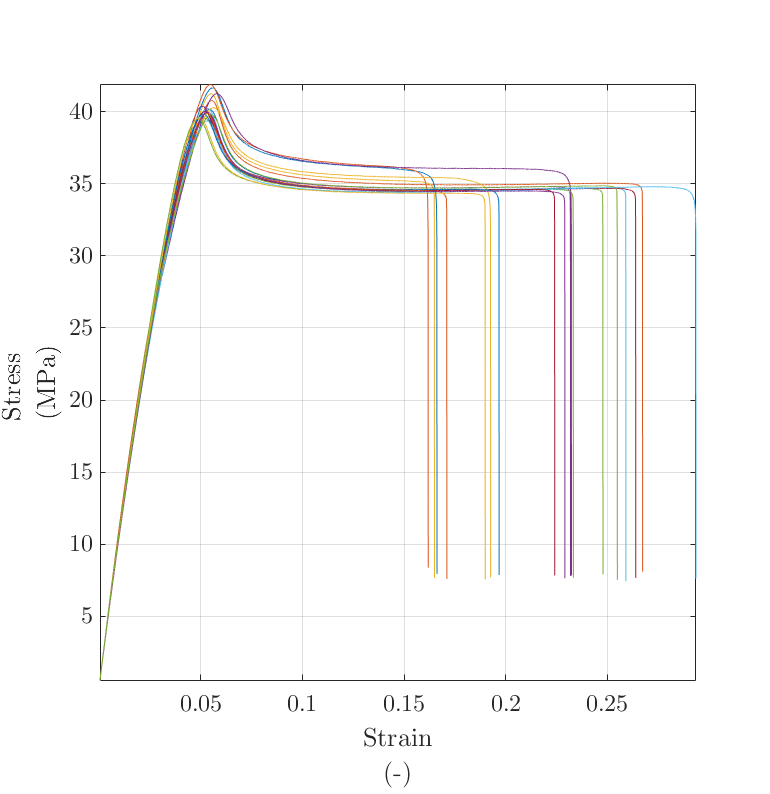
\includegraphics[height=7.5cm, keepaspectratio]{0plot}
	}
	%\hfill
	\subfloat[One test representative of each orientation\label{fig:tenscomp}]{%
	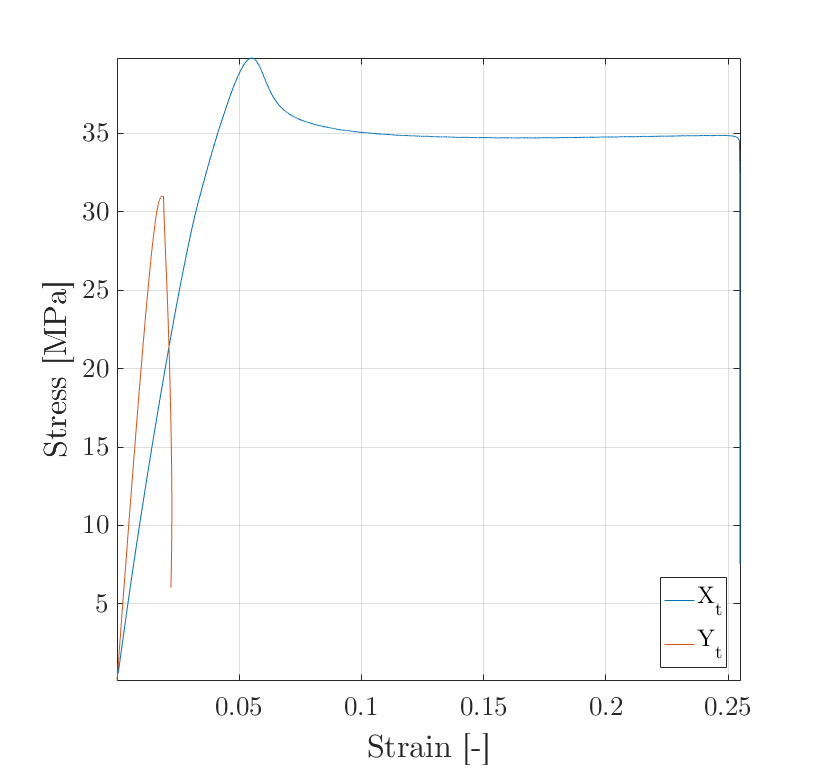
\includegraphics[height=7.3cm, keepaspectratio]{tenscomp}
	}
	\captionsetup{justification=centering} %long caption
	\caption{Comparison of tensile results.} \label{fig:tensComp}
\end{figure}

\begin{figure}[!htbp]
	\center
	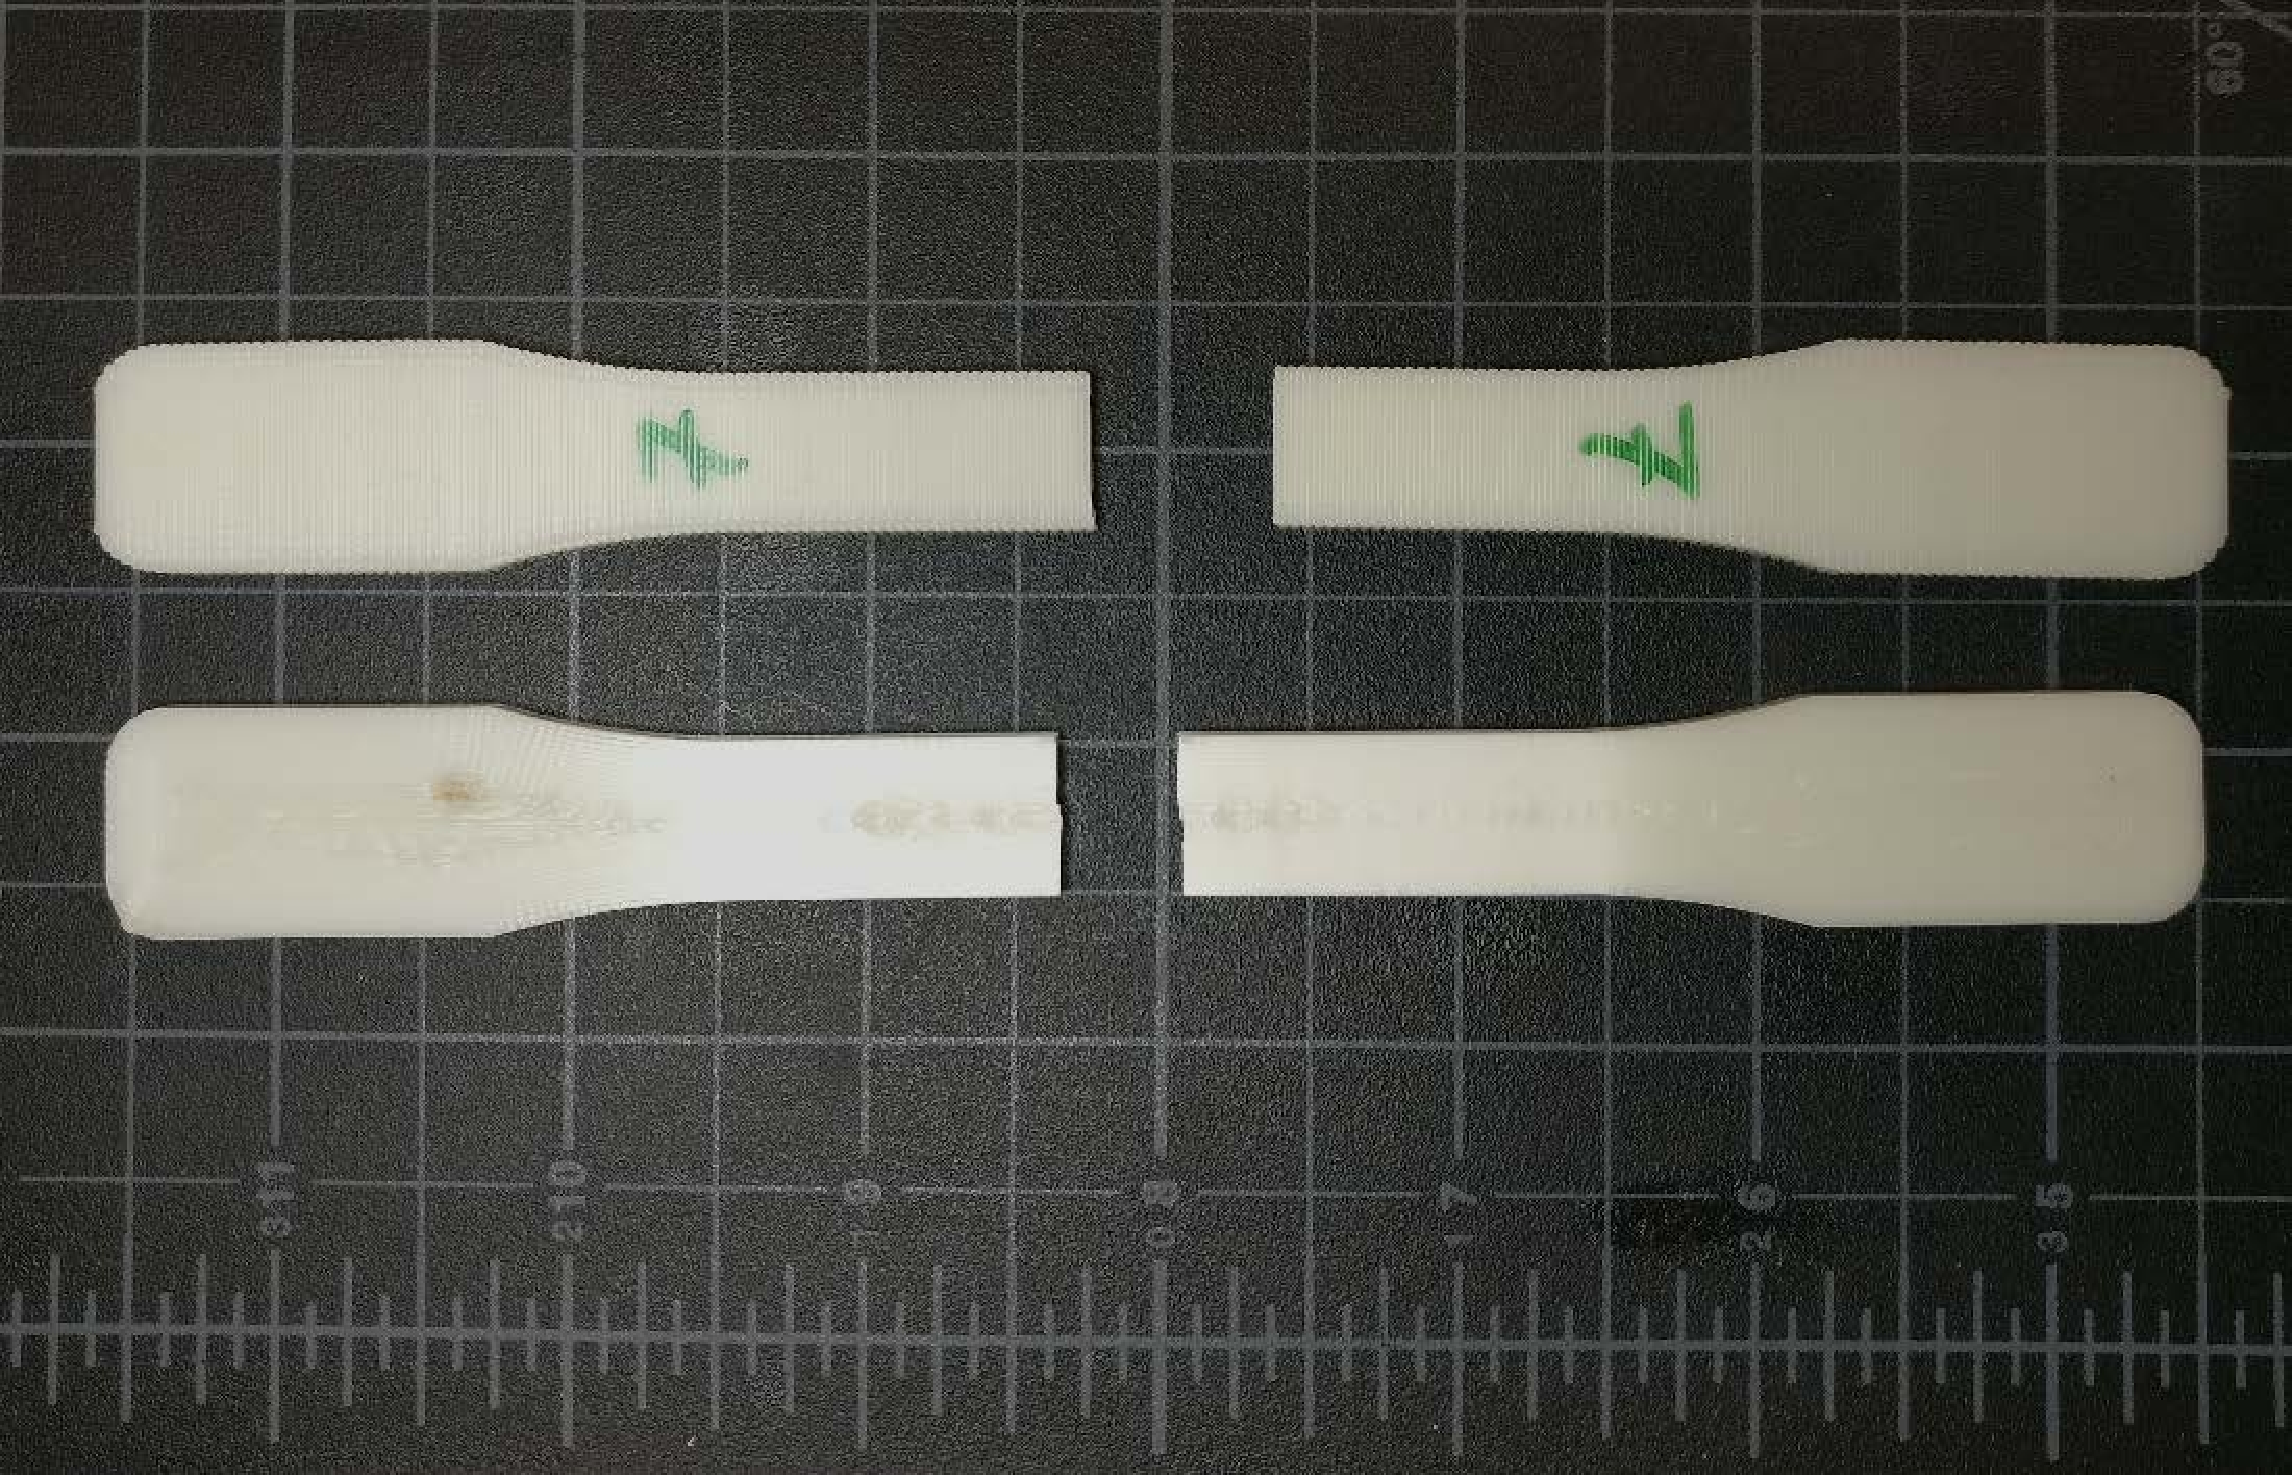
\includegraphics[height=6cm, keepaspectratio]{tenscsomp.pdf}
	\captionsetup{justification=centering} %long caption
	\caption[$X_t$ and $Y_t$ tested samples]{$Y_t$ (top) and $X_t$ (bottom) tested samples. Scale in inches. Note whitening in gage section for $X_t$ specimen.} \label{fig:tensSComp}
\end{figure}

Anderson-Darling tests (ADT) were performed on the results to validate if the data follows a normalized distribution. In the case of $X_t$, the ADT yields a p-value of 0.023. Thus, on a 95\% confidence interval, a normalized distribution can be discarded. This can be seen graphically in the goodness of fit plot, where data points fail to align with the slope that corresponds to a theoretical Gaussian distribution. By contrast, performing the ADT on the $Y_t$ samples fails to reject a normalized distribution using the same confidence interval, offering a p-value of 0.109. %A case could be made for a false negative for $X_t$ and a false positive for $Y_t$, given the relatively small sample size for each data set.
The results from ADT can be seen in Figure \ref{fig:adttens}.

%FIX
\begin{figure}[!htbp]
	\center
	\subfloat[$X_t$ \label{fig:adtxt}]{%
		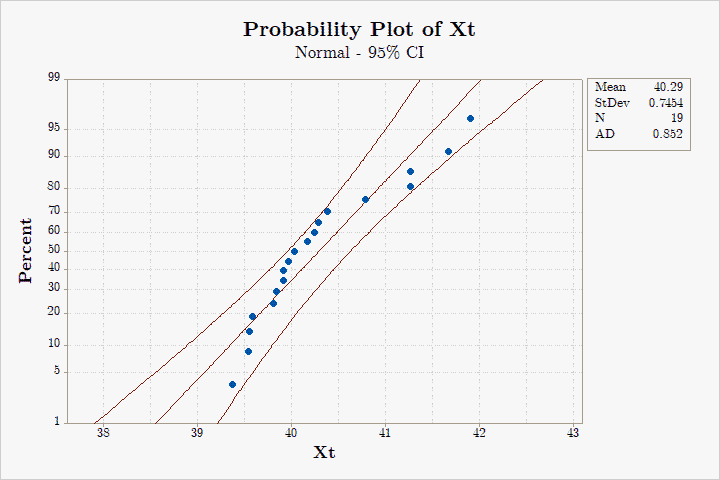
\includegraphics[height=7.5cm, keepaspectratio]{PP_Xt}
	}
	\hfill
	\subfloat[$Y_t$\label{fig:adtyt}]{%
		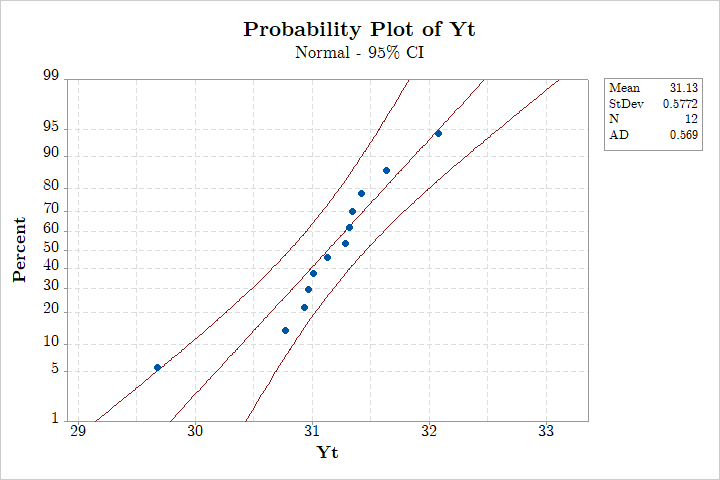
\includegraphics[height=7.5cm, keepaspectratio]{PP_Yt}
	}
	\caption{ADT results for tensile data} \label{fig:adttens}
\end{figure}

\pagebreak
      
\section{Compression Tests} \label{sec:compr}
For the compression tests, a total of 25 samples were produced for each orientation. However, a number of coupons were discarded due to manufacturing defects. Table \ref{tab:comprtab} summarizes the test results.  

\begin{table} [h]
	\centering
	\caption{Summary of compression tests}%ELABORATE
	\begin{tabular}{ c| c c } 
		\toprule
		\textbf{Information} & $X_c$ & $Y_c$\\
		\midrule
		Average [MPa] &43.91  & 57.96\\
		Standard Deviation &3.23  & 1.81\\
		Number of samples &25  & 21\\
		Lowest measurement [MPa] &37.95 &54.93 \\
		Highest measurement [MPa] &48.87 &61.39 \\
		\bottomrule
	\end{tabular}
\label{tab:comprtab}
\end{table}

Surprisingly, both sets of specimens had different failure behavior. The $Y_c$ samples displayed pure ductile behavior through testing. A clear maximum stress can be observed at the yield point in a stress-strain graph, and all samples showed localized whitening and deformation along the center of the specimen. By contrast, the $X_c$ samples showed a considerably lower yield point, cracking sounds were common during testing, and specimens deformed in a way that formed petal-like structures due to contiguous bead delamination. Figure \ref{fig:CompSComp} shows $X_c$ and $Y_c$ samples side by side post testing, where the different failure behavior becomes evident.

\begin{figure}[!htbp]
	\center
	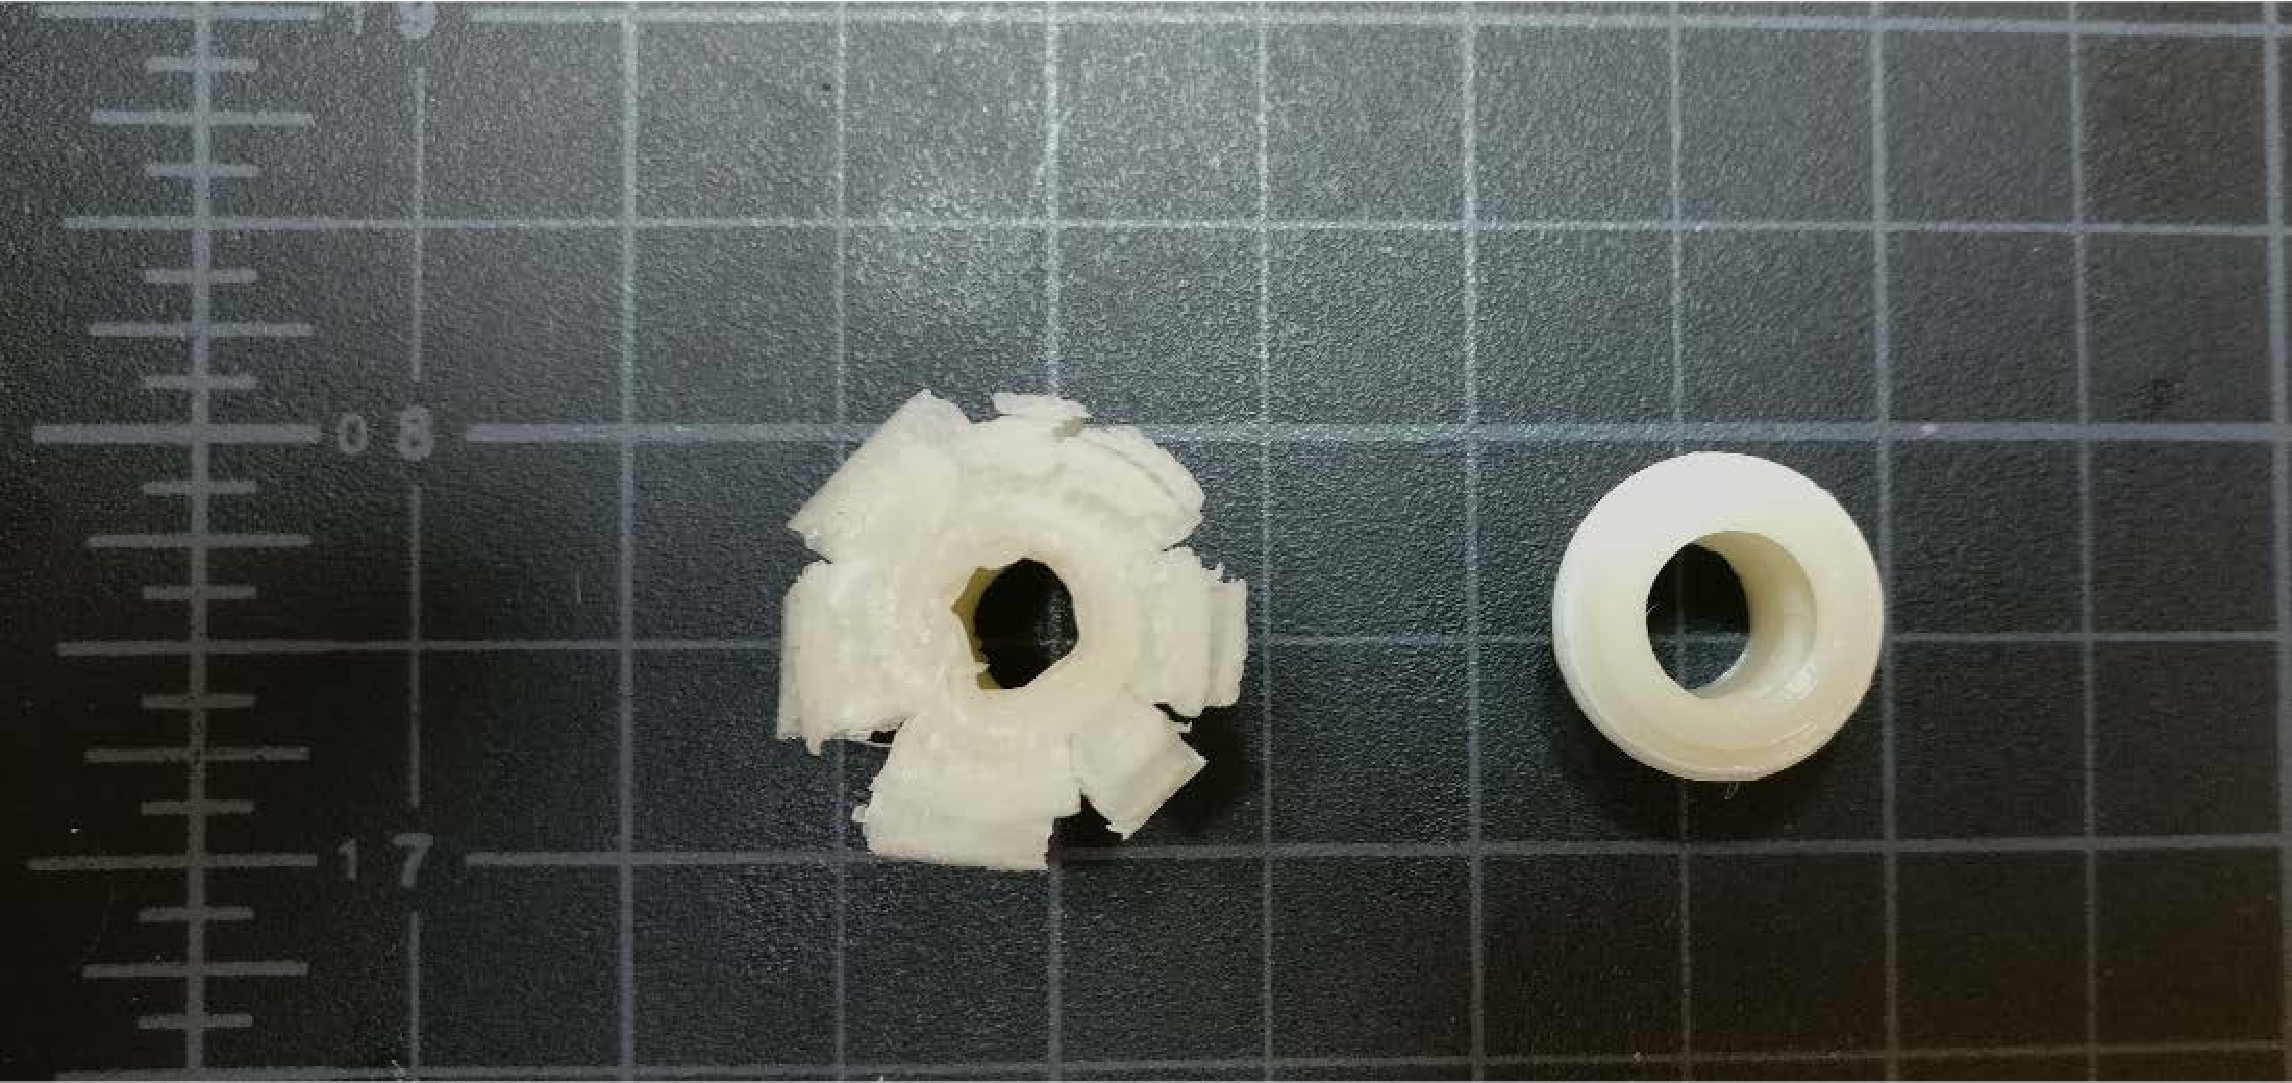
\includegraphics[height=5cm, keepaspectratio]{compscomp.pdf}
	\captionsetup{justification=centering} %long caption
	\caption[$X_c$ and $Y_c$ tested samples]{$X_c$ (left) and $Y_c$ (right) tested samples. Scale in inches. Note petal-like structure of $X_c$ sample.} \label{fig:CompSComp}
\end{figure}

The difference in mechanical behavior can be seen clearly in Figure \ref{fig:comprComp}, where stress-strain curves for $X_c$ and $Y_c$ are compared. Note the erratic behavior of the $X_c$ sample, caused by delamination of adjacent beads.  

\begin{figure}[!htbp]
	\center
	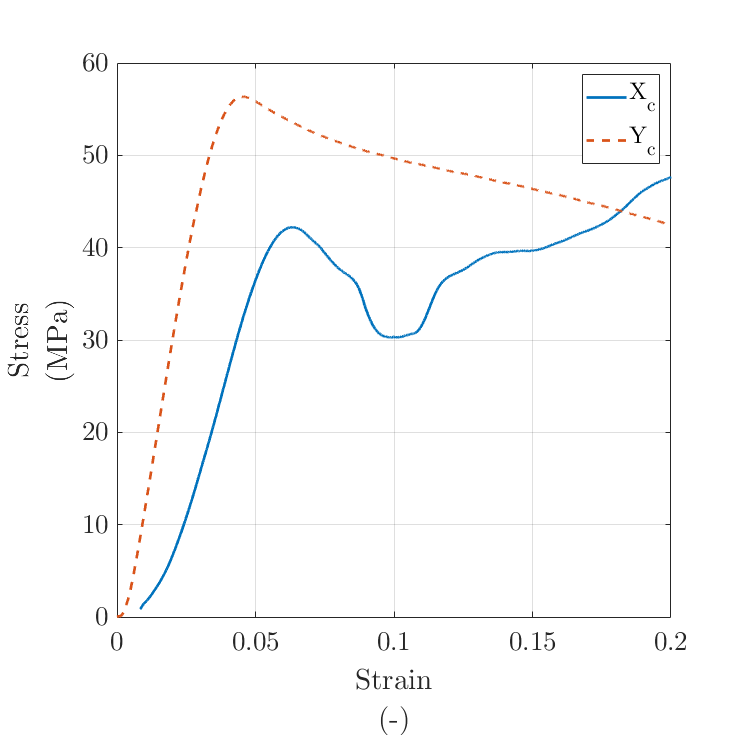
\includegraphics[height=9cm, keepaspectratio]{compresscomp}
	\captionsetup{justification=centering} %long caption
	\caption[Comparison of compression results]{Comparison of compression results. One test representative of each orientation shown.} \label{fig:comprComp}
\end{figure}  

Performing ADT on the data reveals a p-value of 0.072 for $Y_c$, and 0.056 for $X_c$, thus, normalized distributions cannot be discarded on a 95\% confidence interval. These tests can be seen in Figure \ref{fig:adtcomp}.

\begin{figure}[!htbp]
	\center
	\subfloat[$X_c$ \label{fig:adtxc}]{%
		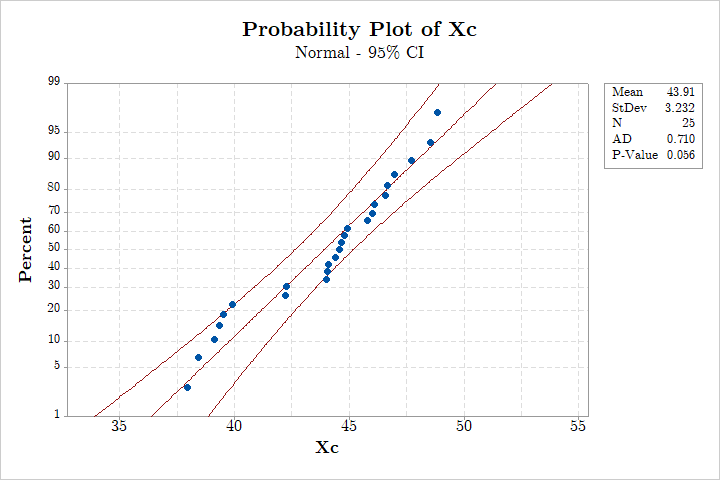
\includegraphics[height=7.5cm, keepaspectratio]{PP_Xc}
	}
	\hfill
	\subfloat[$Y_c$\label{fig:adtyc}]{
		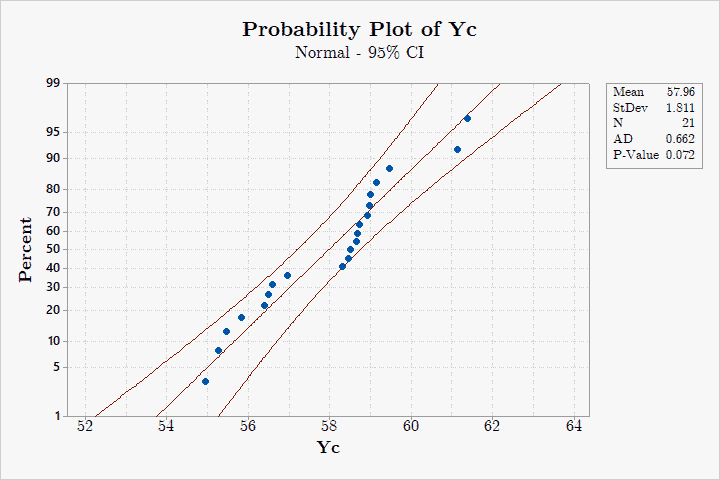
\includegraphics[height=7.5cm, keepaspectratio]{PP_Yc}
	}
	\caption{ADT results for compression tests} \label{fig:adtcomp}
\end{figure}

\newpage
\section{Torsion Tests} \label{sec:torsr}
\subsection{45$^\circ$ orientation} \label{ssec:45r}
A total of 30 samples were produced with a 45$^\circ$ bead orientation, divided evenly for tests in positive and negative shear. As was the case for tensile and compressive tests, a number of specimens had to be discarded due to undesired behavior during testing. A common problem was delamination of the grips, thus requiring the data to be discarded. 

Results showed significant difference in behavior depending on the direction of the applied torque. The $S_{45p}$ samples showed a completely brittle behavior, with fracture occurring between beads, as opposed to ductile failure in the center of the specimen for the $S_{45n}$ coupons. This resulted in an average difference of roughly 17 MPa between both sets of data. Results are summarized in Table \ref{tab:tors45r} and a graph comparing the behavior of both sets of samples can be seen in Figure \ref{fig:45comp}. Note how the positive shear sample fails at low angles in a completely brittle manner. An ADT reveals p-values of 0.841 and 0.133 for the positive and negative shear tests respectively. This implies that normalized distributions can't be discarded on a 95\% confidence interval. 

\begin{table} [h]
	\centering
	\caption{Summary of 45$^\circ$ torsion tests}
\begin{tabular}{ c| c c } 
	\toprule
	\textbf{Information} & $S_{45p}$ & $S_{45n}$\\
	\midrule
	Average [MPa] & 20.80 & 38.17\\
	Standard Deviation & 2.50 & 0.71\\
	Number of samples & 9 & 9\\
	Lowest measurement [MPa] &17.21  & 37.39\\
	Highest measurement [MPa] &24.61 & 39.62\\
	\bottomrule
\end{tabular}
\label{tab:tors45r}
\end{table}

\begin{figure}[!htbp]
	\center
	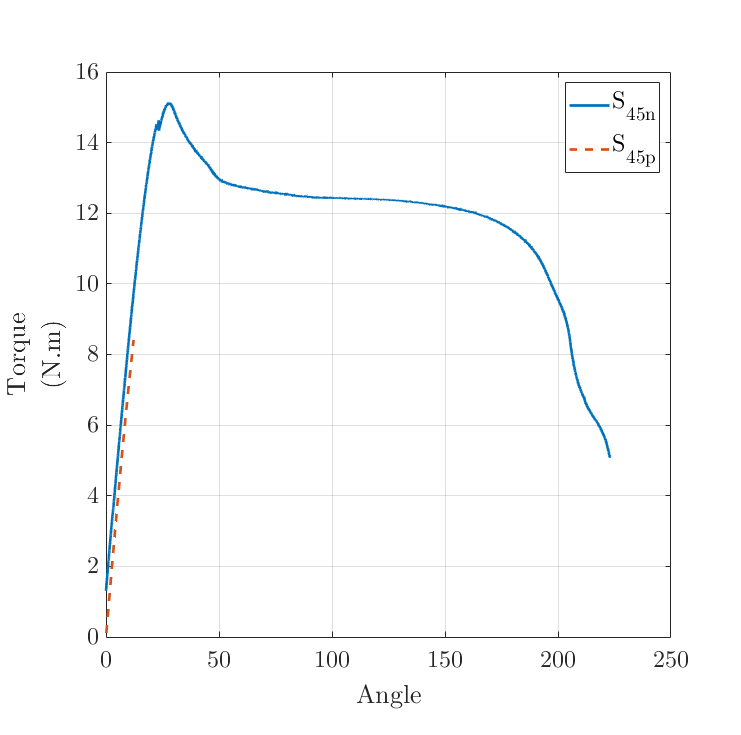
\includegraphics[height=9cm, keepaspectratio]{comp45t}
	\captionsetup{justification=centering} %long caption
	\caption[Comparison of 45$^\circ$ torsion results]{Comparison of 45$^\circ$ torsion results. One test representative of each shear direction shown.} \label{fig:45comp}
\end{figure}

\begin{figure}[!htbp]
	\center
	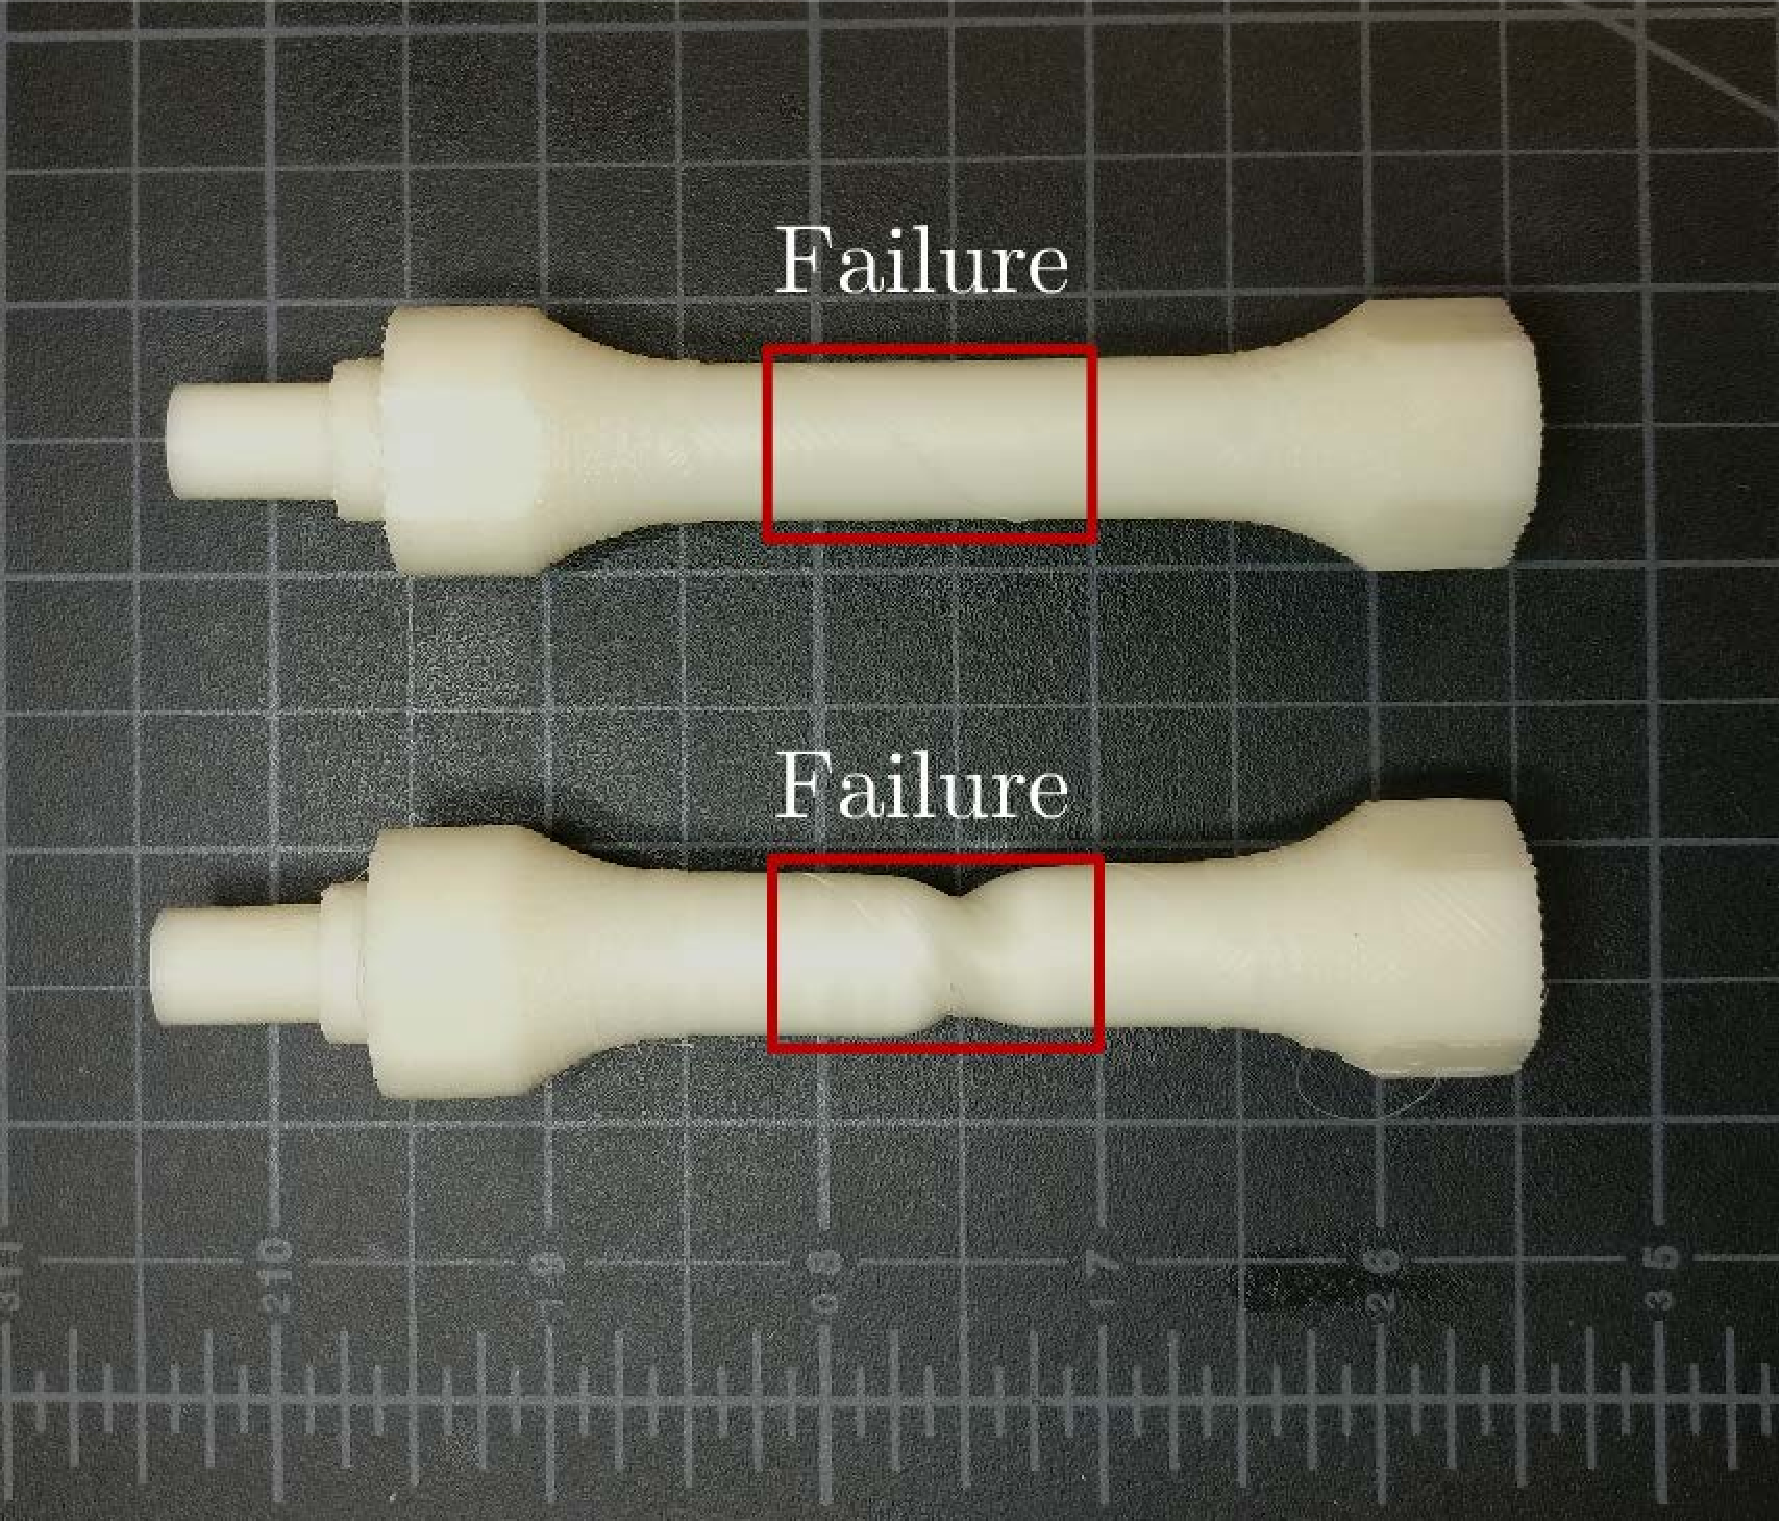
\includegraphics[height=7cm, keepaspectratio]{t45scomp}
	\captionsetup{justification=centering} %long caption
	\caption[Comparison of 45$^\circ$ torsion results]{Comparison of 45$^\circ$ torsion samples. Positive shear (top) caused bead delamination and brittle failure, whereas negative shear (bottom) produced plastic deformation of the gage section} \label{fig:45scomp}
\end{figure}
  
\pagebreak
\subsection{0$^\circ$ and 90$^\circ$ orientation} \label{ssec:090r}

A total of 10 samples were produced for each orientation, however, two were discarded for the 0$^\circ$ raster due to manufacturing defects. Table \ref{tab:tors090r} summarizes the results from the torsion tests. These were used in conjunction with combined loading data to determine shear and axial stress interactions, as well as the maximum shear strength in the $1-2$ plane.

\begin{table} [h]
	\centering
	\caption{Summary of 0$^\circ$ and 90$^\circ$ torsion tests}
\begin{tabular}{ c| c c } 
	\toprule
	\textbf{Information} & $S_{0}$ & $S_{90}$\\
	\midrule
	Average [MPa] &23.35  & 23.41\\
	Standard Deviation &2.78 & 3.21\\
	Number of samples &8  & 10\\
	Lowest measurement [MPa] &18.52  & 18.27\\
	Highest measurement [MPa] &26.56 & 26.60\\
	\bottomrule
\end{tabular}
\label{tab:tors090r}
\end{table}


It can be seen that both orientations produced nearly identical shear stress results. In both cases, samples behaved in an extremely brittle manner, delaminating along contiguous beads. In the case of the 90$^\circ$ orientation, this usually resulted in complete breakage of the specimen. This can be appreciated in Figure \ref{fig:090comptors}, where failure is abrupt and violent in a Torque-Angle graph, as well as in Figure \ref{fig:090ctors}, where tested specimens for both orientations can be seen. Since, practically speaking, both orientations produced the same maximum shear strength result, $S_0$ will be used for further calculations as the parameter $S$ described in Table \ref{tab:testsum}. Performing ADTs on both sets of data reveals p-values of 0.577 and 0.066 for $S_0$ and $S_{90}$ respectively, thus, normalized distributions cannot be discarded in a 95\% confidence interval. The extremely brittle behavior of the samples caused results to have a considerable spread.

\newpage

\begin{figure}[!htbp]
	\center
	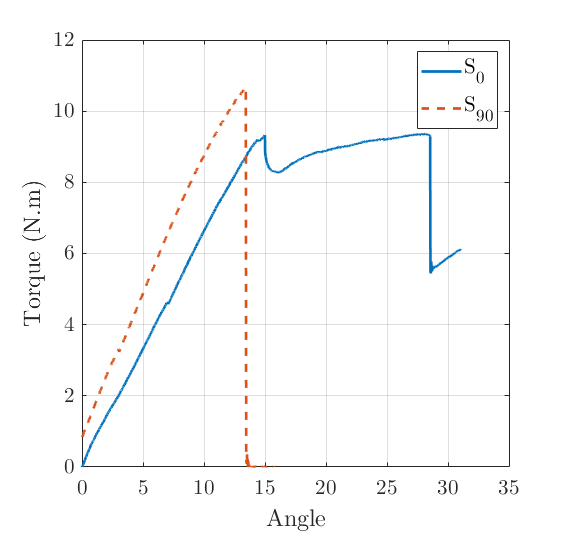
\includegraphics[height=9cm, keepaspectratio]{comp090tors}
	\captionsetup{justification=centering} %long caption
	\caption[Comparison of 0$^\circ$ and 90$^\circ$ torsion results]{Comparison of 0$^\circ$ and 90$^\circ$ torsion results. One test representative of each orientation shown.} \label{fig:090comptors}
\end{figure}

\begin{figure}[!htbp]
	\center
	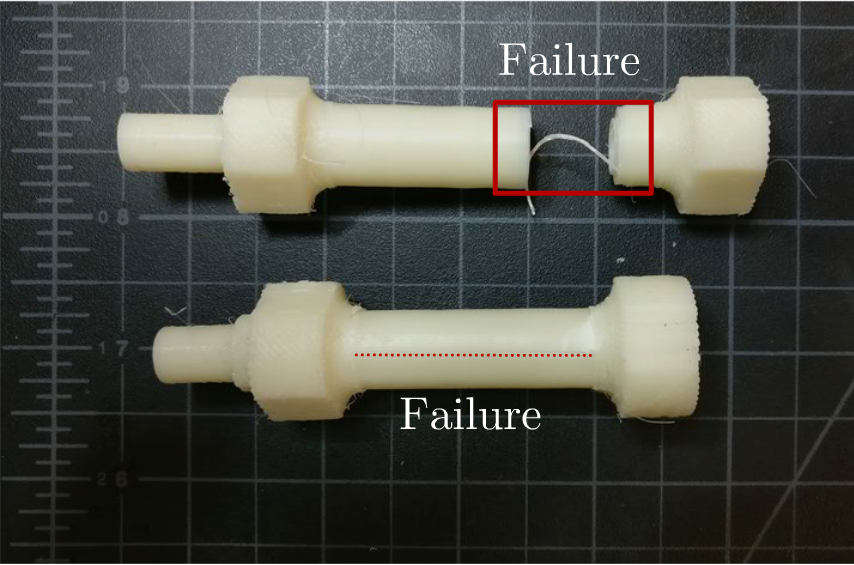
\includegraphics[height=7cm, keepaspectratio]{torscomp090}
	\captionsetup{justification=centering} %long caption
	\caption[Comparison of tested 0$^\circ$ and 90$^\circ$ torsion specimens]{Comparison of tested 0$^\circ$ and 90$^\circ$ torsion specimens. 90$^\circ$ coupons (top) generally separated in parts, whereas 0$^\circ$ specimens (bottom) would delaminate along beads, as highlighted by the red dotted line. Scale in inches} \label{fig:090ctors}
\end{figure}
   
\section{Combined Loading Tests} \label{sec:clr}

Combined loading scenarios involved testing 10 samples in shear and tension, and 10 in shear and compression, totaling 20 samples for each orientation. These results were plotted in the $\tau_{12}-\sigma_{11}$ and $\tau_{12}-\sigma_{22}$ planes to develop the terms $\mu_{1112}$ and $\mu_{2212}$ respectively. Once again, a number of samples was discarded due to manufacturing defects or unwanted failure during testing. A summary of the results can be seen in Table \ref{tab:combl}. Here the superscripts $t$ and $c$ indicate tensile and compressive axial loads respectively, whereas the subscript denotes the orientation of the beads in the torsion specimen. The axial stress was on average 5.8 MPa, attained by hanging a 14.8 kg mass on the setup described in Figure \ref{fig:torscomb}. All samples failed in identical manner to that described in pure shear scenarios. A slight decrease in shear strength can be appreciated for the $S_{90}^t$ scenario.
 
\begin{table} [h]
	\centering
	\caption{Summary of combined loading tests}
	\begin{tabular}{ c| c c c c} 
		\toprule
		\textbf{Information} & $S_{0}^t$ &$S_{0}^c$ & $S_{90}^t$& $S_{90}^c$\\
		\midrule
		Average [MPa] &23.38 &23.13 &20.80 &22.62\\
		Standard Deviation &2.23 &2.98 &2.33 &2.36\\
		Number of samples &8 &10 &10 &9\\
		Lowest measurement [MPa] &19.03 &18.15 &16.37 &18.57\\
		Highest measurement [MPa] &26.46 &26.28 &23.93 &26.50\\
		\bottomrule
	\end{tabular}
	\label{tab:combl}
\end{table}
 
\section{Development of the Failure Surface} \label{sec:fsc}

The failure surface calculations were performed using MATLAB\textregistered~code based on previous work by Obst \emph{et al.} \cite{Obst2018} and the mathematical relations shown in Chapter \ref{ch:oocrit}. This code can be found in Appendix \ref{ch:fsurfcode} for reference. Appendices \ref{ch:data} and \ref{ch:surf} include MATLAB\textregistered~code that recreates the data and envelopes shown here.  

Calculations were based on the average values obtained from the mechanical tests in order to incorporate a probabilistic approach as developed by Zaitsev, Pashkov and Strelyaev \cite{Zaitsev1975}. In practice, this signifies that the condition $f=1$ in Equation \ref{eq:GKCfinal} is equivalent to a probability of part failure equal to 50\%.

Starting with the $\sigma_{11}$-$\sigma_{22}$ plane, it can be seen that the failure envelope has a slight tilt, agreeing with the difference observed between compressive and tensile strengths in both directions, as well as the difference in behavior for the $S_{45}$ tests. Refer to Figure~\ref{fig:1122plane} for a graph showing the calculated failure envelope, including the experimental data for reference.

\pagebreak

\begin{figure}[!htbp]
	\center
	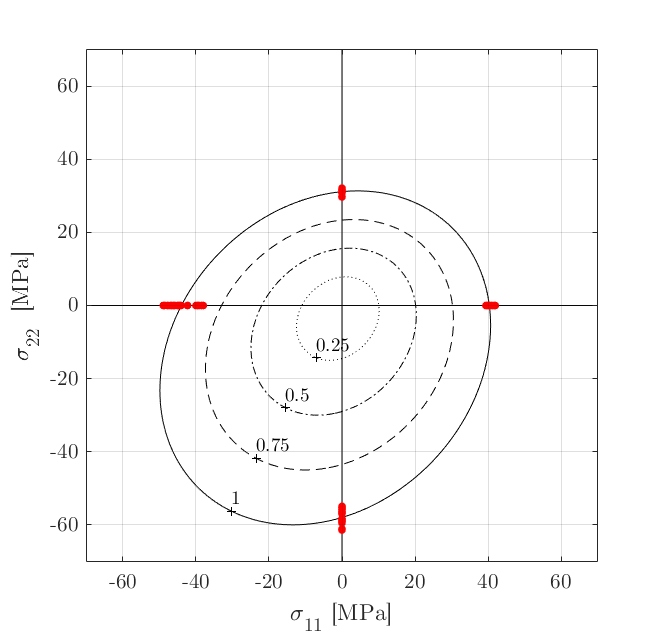
\includegraphics[width=0.9\linewidth, keepaspectratio]{11_22plane}
	\captionsetup{justification=centering} %long caption
	\caption[failure envelope in the $\sigma_{11}$-$\sigma_{22}$ plane]{$\sigma_{11}$-$\sigma_{22}$ plane including data of $X_t$, $X_c$, $Y_t$ and $Y_c$ tests. Graph shows calculated f values of 1, 0.75, 0.50 and 0.25 to illustrate safety factors of 1, 4/3, 2 and 4 respectively.} \label{fig:1122plane}
\end{figure}

It can be seen from the tilt of the envelope that there is an interaction between the transverse and longitudinal stresses. Figure \ref{fig:1122plane} indicates that FFF parts produced with the print parameters used should show strengthening when loaded bi-axially in compression. Further experimental work would be of interest to compare bi-axial compression test data to this result. Computing all tensorial components associated with the  $\sigma_{11}$-$\sigma_{22}$ plane results in Table \ref{tab:1122calc}. Note how $F_{1122}$ is negative and in the same order of magnitude as $F_{1111}$ and $F_{2222}$. 


\begin{table} [h]
	\centering
	\caption{Tensorial components obtained from tests in the $\sigma_{11}$-$\sigma_{22}$ plane}
	\begin{tabular}{ c c } 
		\toprule
		\textbf{Component} & \textbf{Value} \\
		\midrule
		$F_{11}$ & 1.023$\times 10^{-3}$\\ 
		$F_{1111}$ & 5.663$\times 10^{-4}$\\ 
		$F_{22}$ & 7.435$\times 10^{-3}$\\ 
		$F_{2222}$ & 6.095$\times 10^{-4}$\\ 
		$F_{1122}$ & -1.017$\times 10^{-4}$\\ 
		\bottomrule
	\end{tabular}
	\label{tab:1122calc}
\end{table}  

Using the results from combined loading tests plotted in the $11-12$ and $22-12$ planes allows the calculation of the slopes $\mu^{1112}$ and  $\mu^{2212}$. Beginning with the $11-12$ plane, it can be seen that the averages for $S_{0}$, $S_{0}^c$  and $S_{0}^t$ were extremely close to each other, and the spread of the data occludes any trends. Using the averages for $S_{0}$ and $S_{0}^t$ to calculate the slope yields $\mu^{1112}$ equal to $5.2\times 10^{-3}$, a value that's practically zero. Using this parameter, the failure surface shown in Figure \ref{fig:1112plane} can be obtained. A dashed line representing $\mu^{1112}$ is added for reference.

\pagebreak

\begin{figure}[!htbp]
	\center
	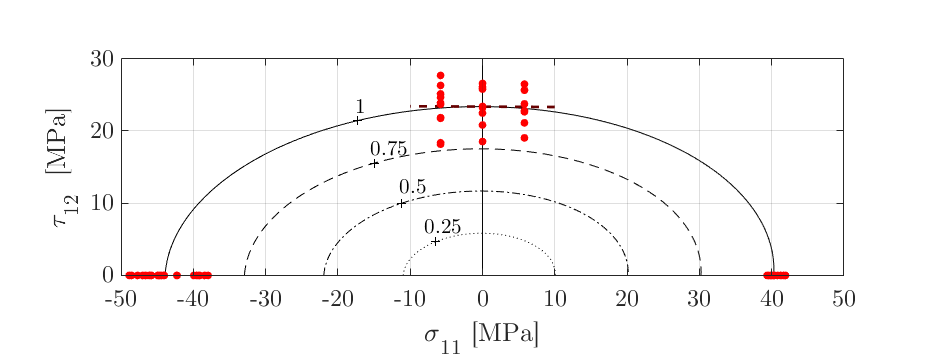
\includegraphics[width=\linewidth, keepaspectratio]{11_12plane}
	\captionsetup{justification=centering} %long caption
	\caption[failure envelope in the $\sigma_{11}$-$\tau_{12}$ plane]{$\sigma_{11}$-$\tau_{12}$ plane including data of $X_t$, $X_c$, $S_{0}$, $S_{0}^t$ and $S_{0}^c$ tests. Graph shows calculated f values of 1, 0.75, 0.50 and 0.25 to illustrate safety factors of 1, 4/3, 2 and 4 respectively.} \label{fig:1112plane}
\end{figure}

The $22-12$ plane by comparison reveals a considerable slope. It can be seen through the use of combined loads that there is a slight decrease in the shear strength of the specimens when a tensile load is applied in the $2-2$ direction. A slope of -0.2 was chosen for $\mu^{2212}$. Figure \ref{fig:2212plane} shows the resulting surface with the data and a line with a slope of -0.2 overlaid for reference.

\begin{figure}[!htbp]
	\center
	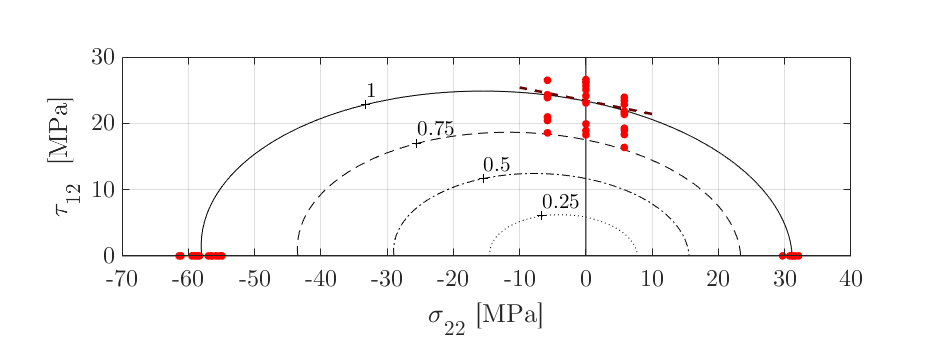
\includegraphics[width=\linewidth, keepaspectratio]{22_12plane}
	\captionsetup{justification=centering} %long caption
	\caption[failure envelope in the $\sigma_{22}$-$\tau_{12}$ plane]{$\sigma_{22}$-$\tau_{12}$ plane including data of $Y_t$, $Y_c$, $S_{90}$, $S_{90}^t$ and $S_{90}^c$ tests. Graph shows calculated f values of 1, 0.75, 0.50 and 0.25 to illustrate safety factors of 1, 4/3, 2 and 4 respectively.} \label{fig:2212plane}
\end{figure}

Finally, using the chosen values of $\mu^{1112}$ and $\mu^{2212}$, the remaining parameters of the failure surface can be calculated. These are available in Table \ref{tab:remcalc}. These values were then used to plot the complete failure surface shown in \ref{fig:fullfs}.

\begin{table} [!htbp]
	\centering
	\caption{Tensorial components obtained from tests in the $\sigma_{11}$-$\tau_{12}$ and $\sigma_{22}$-$\tau_{12}$ planes}
	\begin{tabular}{ c c } 
		\toprule
		\textbf{Component} & \textbf{Value} \\
		\midrule
		$F_{12}$ & 0\\
		$F_{1212}$ & 1.834$\times 10^{-3}$\\
		$F_{1112}$ & -3.428$\times 10^{-5}$\\
		$F_{2212}$ & 4.841$\times 10^{-5}$\\
		\bottomrule
	\end{tabular}
	\label{tab:remcalc}
\end{table}  

\begin{figure}[!htbp]
	\center
	\includegraphics[width=\linewidth, keepaspectratio]{final_surface}
	\captionsetup{justification=centering} %long caption
	\caption[Complete Failure Surface]{Complete Failure Surface plotted with calculated f values of 1, 0.75, 0.50 and 0.25 to illustrate safety factors of 1, 4/3, 2 and 4 respectively.} \label{fig:fullfs}
\end{figure} 


% Nomenclature introduced in this chapter:
\nomenclature[A]{ADT}{Anderson-Darling Test}% 

% Symbols introduced in this chapter:
%\nomenclature[S]{$\epsilon$}{Engineering Strain \nomunit{$-$}}%
\end{document}